\chapter{Introduction}
\begin{figure}[h!]
  \centering
    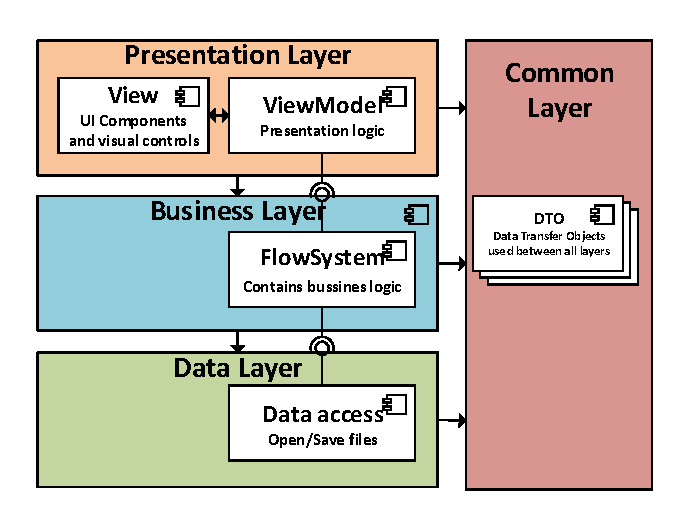
\includegraphics{figures/SystemOverview.pdf}
  \caption{Overview of the system.}
  \label{fig:systemoverview}
\end{figure}

\section{Abstraction layers}
The system is divided in layers to make the software more modular. For example the "Data Layer" could be replaced to make it work with a Database, for now the application only works with the file system. Abstraction layers are used to follow Separation of Concerns from SOLID principals. The components of figure \ref{fig:systemoverview} know about each other through Dependency Injection whereby the components don't really know about each other to prevent the code from being glued together. The code is more testable since it is modular.

\subsection{Common Layer}
The Common Layer is referenced by all the other layers. It contains DTO's which are objects transferred between all the layers. The objects only contain data and don't have any behavior, so the objects are really stupid and have no logic.

\subsection{Presentation Layer}
The presentation layer handles the UI of the application, this layer doesn't have any business logic. WPF is used for handling the graphics since it allows an MVVM pattern to be implemented see figure \ref{fig:mvvm}. The Presentation Layer only contains the View and the ViewModel, the model is in the Bussines Layer,
\begin{figure}[h!]
  \centering
    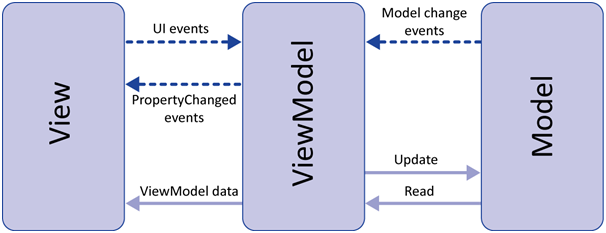
\includegraphics[scale=0.8]{figures/mvvm.png}
  \caption{Model View ViewModel}
  \label{fig:mvvm}
\end{figure}

\subsection{Business Layer}
The business layer contains the business logic of the program. Business logic include calculating the flow through the network.

\subsection{Data Layer}
The data layer contains the logic to read and write the flow network to a file.